\section*{Качество классификации: Precision, Recall}

В задаче классификации \textbf{precision} (точность) и \textbf{recall} (полнота) являются ключевыми метриками для оценки качества предсказания, особенно в задачах с несбалансированными классами.

\subsection*{Определения}

Рассмотрим бинарную классификацию, то есть объект может быть либо положительным (positive), либо отрицательным (negative), и определим:

\begin{itemize}
    \item $TP$ (\textit{True Positives}) — количество объектов, правильно классифицированных как положительные.
    \item $FP$ (\textit{False Positives}) — количество объектов, ошибочно классифицированных как положительные.
    \item $FN$ (\textit{False Negatives}) — количество объектов, ошибочно классифицированных как отрицательные.
    \item $TN$ (\textit{True Negatives}) — количество объектов, правильно классифицированных как отрицательные.
\end{itemize}

На основе этих величин вычисляются:

\begin{enumerate}
    \item \textbf{Precision:}
    \[
    \text{Precision} = \frac{TP}{TP + FP}.
    \]
    Precision показывает долю истинно положительных объектов среди всех объектов, классифицированных как положительные.

    \item \textbf{Recall:}
    \[
    \text{Recall} = \frac{TP}{TP + FN}.
    \]
    Recall показывает долю истинно положительных объектов среди всех реально положительных объектов.
\end{enumerate}

\begin{figure}[ht!]
	\centering
	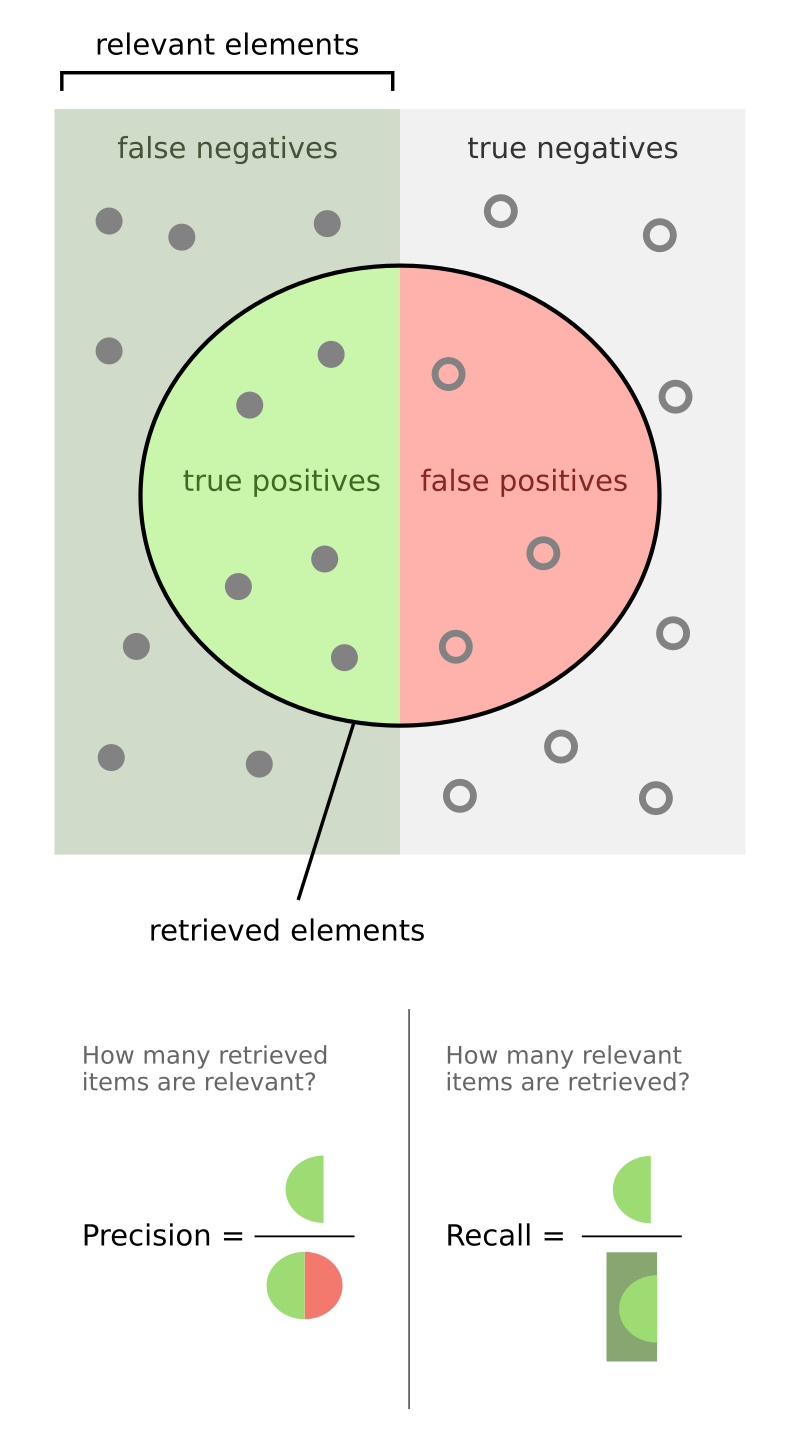
\includegraphics[width=0.65\linewidth]{chapters/model_selection/images/Precisionrecall.png}
\end{figure}

\subsection*{Интуитивное объяснение}

\begin{itemize}
    \item \textbf{Precision}: Насколько «точен» алгоритм, когда он говорит, что объект положительный? Если precision высокое, значит, ложные срабатывания ($FP$) минимальны.
    \item \textbf{Recall}: Насколько хорошо алгоритм находит все положительные объекты? Если recall высокое, значит, пропущенные положительные объекты ($FN$) минимальны.
\end{itemize}

\subsection*{Пример}

Классический пример использования метрик precision и recall - задача поиска спама на почте. В этом случае спам - положительная категория. Пусть у нас есть 100 писем, из которых 40 писем — спам, 60 писем — не спам.

Алгоритм классифицировал 50 писем как спам, из которых 30 писем действительно оказались спамом, а остальные 20 писем были ошибочно классифицированы как спам. Вычислим в этом случае precision и recall:

\begin{itemize}
    \item \textbf{Precision:}
    \[
    \text{Precision} = \frac{TP}{TP + FP} = \frac{30}{30 + 20} = 0.6.
    \]

    \item \textbf{Recall:}
    \[
    \text{Recall} = \frac{TP}{TP + FN} = \frac{30}{30 + 10} = 0.75.
    \]
\end{itemize}

\subsection*{Баланс между precision и recall}

Модель для каждого объекта на входе генерирует какое-то число на выходе. В простейшем варианте объект классифицируется как положительный, если это число больше некого выставленного порога, и как отрицательный в обратном случае. Увеличивая порог классификации, мы снижает количество False Positive объектов, потому precision увеличивается. При этом количество "незамеченных" моделью положительных объектов тоже вырастет, поэтому recall снизится. При уменьшении порога будет наблюдаться обратный эффект. Обычно стараются добиться компромиссного значения, при котором precision и recall оба принимают удовлетворительные значения. В некоторых случаях одна из метрик важнее другой:

\begin{itemize}
    \item Детекция спам-рассылок. В этом случае мы чаще всего не хотим пометить важные письма, как спам. Поэтому нужно снизить False Positive - важнее precision.
    \item Первичного выявление заболевания. Мы не хотим пропустить пациентов, которые на самом деле больны, только потому что модель сказала обратное. Поэтому важно снизить False Negative - в этом случае важнее recall. 
\end{itemize}

\subsection*{Интуитивное объяснение}

Если при получении положительного ответа от модели мы предпринимаем какое-либо действие, то precision важнее, когда действие обходится дорого, а recall важнее, когда бездействие обходится дорого. В примерах выше: помещение важного письма в папку "спам" (действие) может привести к финансовым потерям, а пропуск реального спама во "входящие" (бездействие) лишь заставит человека сделать это вручную. С другой стороны, при ложноположительном диагнозе человек пройдёт дополнительные анализы (действие), а ложноотрицательный может стоить ему жизни (бездействие).

\begin{figure}[ht!]
	\centering
	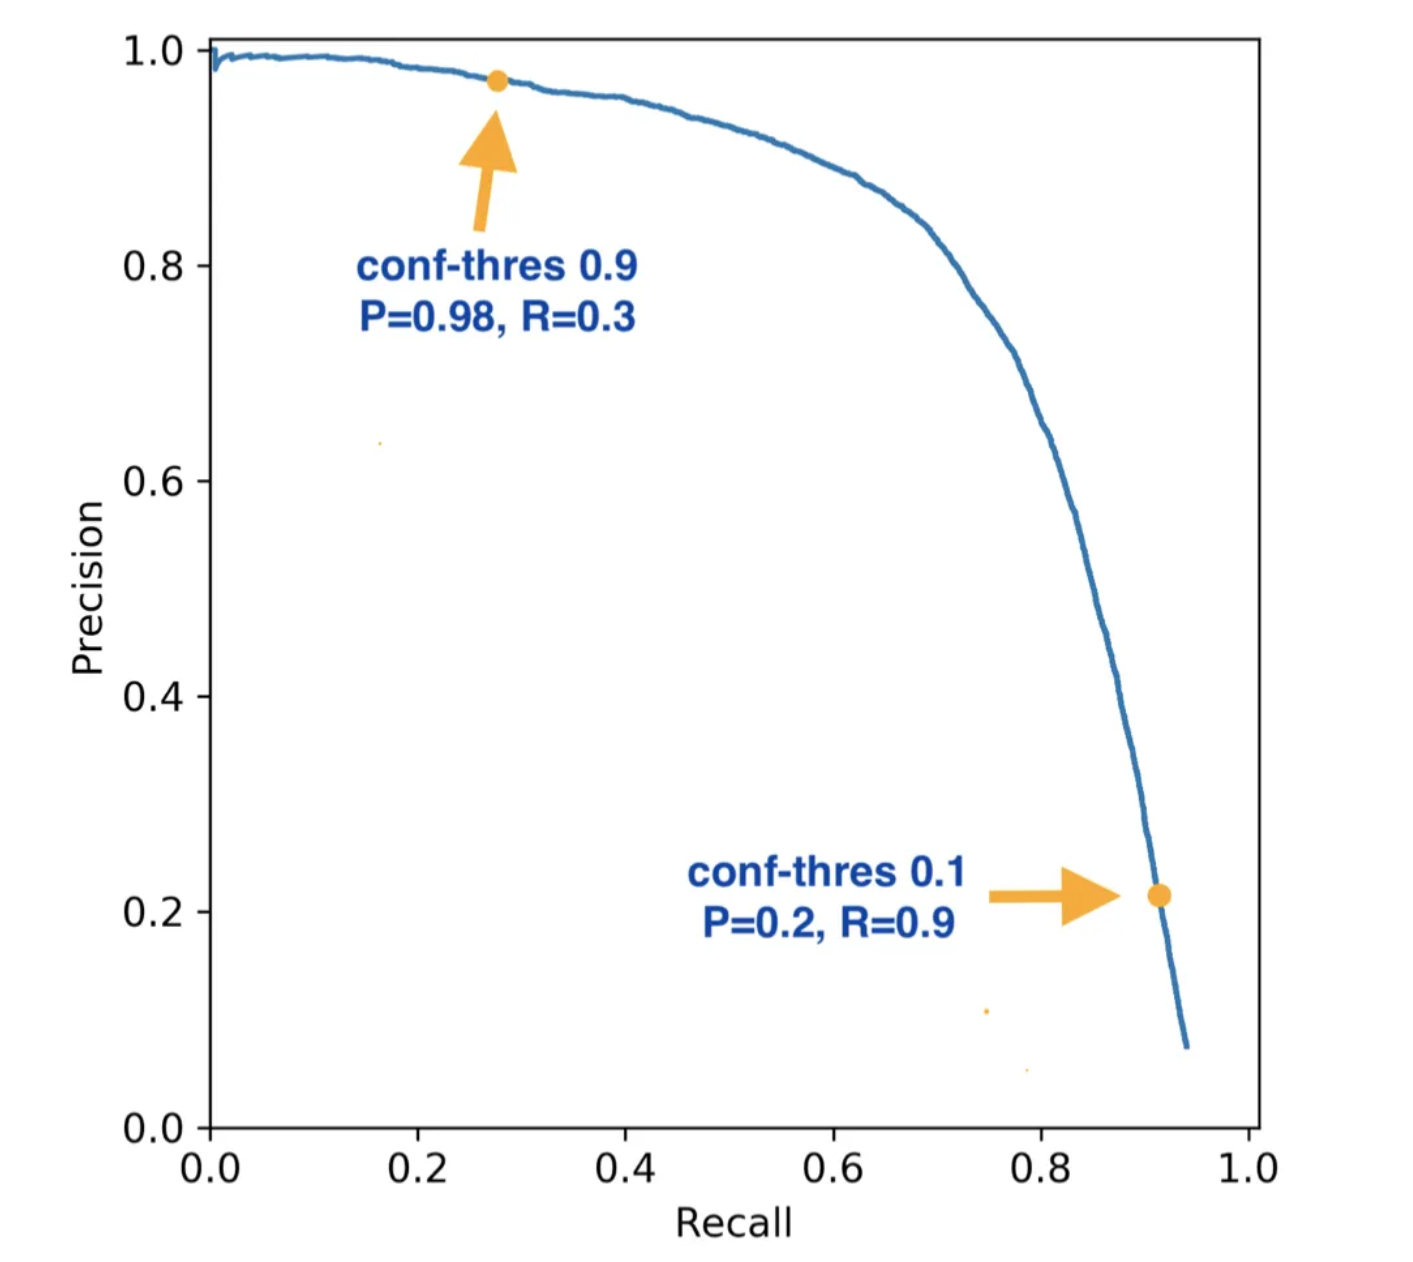
\includegraphics[width=0.65\linewidth]{chapters/model_selection/images/Precisionrecallcurve.png}
\end{figure}

\bigskip
\bigskip

Для того, чтобы изобразить баланс между двумя метриками, строят precision-recall кривую. Точки на ней соответствуют разным значениям порога.

\subsection*{F-метрика (дополнительно)}

Часто для оценки общего качества модели используется метрика $F$-мера, которая является гармоническим средним между precision и recall с параметром $\beta$:
\[
F_{\beta} = (1 + \beta^2) \cdot \frac{\text{Precision} \cdot \text{Recall}}{\beta^2 \cdot \text{Precision} + \text{Recall}}.
\]
Из формулы понятно, что $\beta$ определяет, насколько recall важнее по сравнению с precision. Наиболее часто используется $F_1$-мера:
\[
F_1 = 2 \cdot \frac{\text{Precision} \cdot \text{Recall}}{\text{Precision} + \text{Recall}}.
\]

\subsection*{Задачи}

\subsection*{Задача 1: Простейшая модель}

Как будет выглядеть precision-recall кривая у простейшей модели, которая для любого объекта делает positive предсказание с вероятностью $1-t$ (при $t = 1$ все предсказания отрицательные, при $t = 0.5$ - половина)? Как в этом случае и с использованием метрик precision и recall подбирать параметр $t$, чтобы добиться лучшей работы модели?

\textbf{Ответ:}

В координатах ($recall$, $precision$) - отрезок с концами в (0, $\alpha$) и (1, $\alpha$), где $\alpha$ - доля положительных объектов в выборке (горизонтальный отрезок). Объяснение состоит в том, что доля $TP$ равна $\alpha (1-t)$, доля $TP + FN$ равна $\alpha$, а доля $TP + FP$ равна $(1-t)$. Таким образом, значения precision и recall не зависят от параметра $t$, то есть его изменение не изменит качество модели в этих метриках.

\subsection*{Задача 2: Дисбаланс классов}

Какая из метрик -- precision или recall -- будет больше в случае сильного дисбаланса классов на тестовой выборке (рассмотреть оба случая), если известно, что модель обучалась на сбалансированном датасете?

\textbf{Ответ:}

Если положительных объектов значительно меньше, чем отрицательных, то recall будет больше. Это связано с тем, что сбалансированная модель в этом случае будет допускать много False Positive ошибок. При обратном дисбалансе precision будет больше из-за большого количества False Negative ошибок.

\subsection*{Задача 3: Мошеннические транзакции}

Финансовая компания использует алгоритм для выявления мошеннических транзакций. Из 10,000 проверенных транзакций 500 транзакций являются мошенническими, 9,500 транзакций являются легитимными.

Алгоритм определил 600 транзакций как мошеннические, из которых 400 действительно оказались мошенническими.

\begin{enumerate}
    \item Вычислите $F_1$-меру.
    \item Насколько может измениться $F_1$-мера, если алгоритм пометит ещё 50 транзакций как мошеннические, в зависимости от того, являются они на самом деле мошенническими или нет?
\end{enumerate}

\textbf{Решение:}
Найдём precision и recall.
\begin{itemize}
    \item
    \[
    \text{$precision$} = \frac{400}{400 + 200} = \frac{400}{600} \approx 0.667.
    \]
    \item
    \[
    \text{$recall$} = \frac{400}{400 + 100} = \frac{400}{500} = 0.8.
    \]
    \item
    \[
    \text{$F_1$-score} = 2\frac{precision\cdot recall}{precision + recall} = 2\frac{0.667\cdot 0.8}{0.667 + 0.8} \approx 0.722
    \]

\end{itemize}

Обозначим за $\alpha$ долю тех новых помеченных транзакций, которые на самом деле являются мошенническими ($0 \le \alpha \le 1$). Понятно, что $TP$ увеличится на $50\alpha$, $FN$ уменьшится на $50\alpha$, а $TP + FP$ станет равным 650. Посчитаем precision, recall, изменение $F_1$-score в общем случае:

\begin{itemize}
    \item
    \[
    \text{$precision$} = \frac{400 + 50\alpha}{650}.
    \]
    \item
    \[
    \text{$recall$} = \frac{400 + 50\alpha}{500}.
    \]
    \item
    \[
    \text{$F_1$-score} = \frac{16 + 2\alpha}{23} \approx 0.696 + 0.087\alpha
    \]
    \item
    \[
    \text{$\Delta F_1$-score} \approx 0.696 + 0.087\alpha - 0.722 = -0.026 + 0.087\alpha
    \]
\end{itemize}

Таким образом, $F_1$-мера уменьшится на -0.026 если все новые помеченные транзакции на самом деле легитимные, увеличится на 0.061, если они все на самом деле мошеннические. Заметим, что $F_1$-мера останется неизменной, если $\alpha = \frac{1}{3}$, то есть изначальная доля ложноположительных среди всех помеченных.


\section{Применение обоснованности при выборе модели}

\subsection{Мотивация введения понятия обоснованности}

В процессе анализа данных и построения моделей мы сталкиваемся с необходимостью выбора наилучшей модели среди множества возможных вариантов. Однако традиционные подходы, такие как минимизация ошибки на обучающей выборке, могут привести к переобучению и, следовательно, плохой обобщаемости модели на новых данных. Чтобы избежать этого, необходимо оценивать качество модели не только по ее способности предсказывать известные данные, но и по тому, насколько она совместима с предполагаемым распределением данных.

Именно здесь возникает понятие обоснованности, которое помогает нам сравнивать разные модели на основе вероятности того, что они могли бы породить наблюдаемые данные. В отличие от других критериев, таких как точность на тестовой выборке или ошибка обучения, обоснованность учитывает как сложность модели, так и ее способность объяснять данные без чрезмерного усложнения.

\subsection{Определение обоснованности}

Обоснованность (или marginal likelihood) — это вероятность наблюдаемых данных при условии выбранной модели. Она выражается следующим образом:

\begin{equation}
    p(\mathbf{X} \mid \mathcal{M}) = \int p(\mathbf{X} \mid \boldsymbol{\theta}, \mathcal{M}) \, p(\boldsymbol{\theta} \mid \mathcal{M}) \, d\boldsymbol{\theta}
\end{equation}

Где:$\mathbf{X}$ — наблюдаемая выборка данных,$\mathcal{M}$ — рассматриваемая модель, $\boldsymbol{\theta}$ — вектор параметров модели, $p(\mathbf{X} \mid \boldsymbol{\theta}, \mathcal{M})$ — функция правдоподобия данных при фиксированных значениях параметров, $p(\boldsymbol{\theta} \mid \mathcal{M})$ — априорное распределение параметров модели.

Интеграция по параметрам $\boldsymbol{\theta}$ означает усреднение правдоподобия по всем возможным значениям параметров, взвешенным согласно их априорной вероятности. Таким образом, обоснованность показывает, насколько хорошо модель объясняет данные, учитывая все возможные комбинации значений параметров.

\subsubsection{Задача 1: Обоснованность для модели линейной регрессии}
Пусть имеется модель линейной регрессии с нормальным шумом
\begin{equation*}
 \mathbf{y} = \mathbf{X}\mathbf{w} + \boldsymbol{\varepsilon}, \quad \boldsymbol{\varepsilon} \sim \mathcal{N}(0, \sigma^2 \mathbf{I}),
\end{equation*}
где $\sigma^2$ --- известно, и априорным распределением на $\mathbf{w}$ $p(\mathbf{w}) = \mathcal{N}(\mathbf{w} \mid \mathbf{m}, \alpha^2 \mathbf{I}))$, где $\mathbf{m}$ и $\alpha$ ---
неизвестные гиперпараметры.

Найдите обоснованность модели $p(\mathbf{y} \mid \mathbf{X}, \mathbf{m}, \alpha)$ с точностью до константы.

\subsubsection*{Решение}

Функция правдоподобия для нашей модели линейной регрессии с нормальными ошибками записывается как:

\begin{align*}
 p(\mathbf{y} \mid \mathbf{X}, \mathbf{w}, \sigma^2) &= \mathcal{N}(\mathbf{y} \mid \mathbf{X}\mathbf{w}, \sigma^2 \mathbf{I}) \\
 &\propto \exp\left(-\frac{1}{2\sigma^2}(\mathbf{y} - \mathbf{X}\mathbf{w})^\top(\mathbf{y} - \mathbf{X}\mathbf{w})\right)
\end{align*}

где $N$ — число наблюдений, а $\mathbf{I}$ — единичная матрица размера $N \times N$.

Априорное распределение для $\mathbf{w}$:

\begin{align*}
 p(\mathbf{w} \mid \mathbf{m}, \alpha^2) &= \mathcal{N}(\mathbf{w} \mid \mathbf{m}, \alpha^2 \mathbf{I}) \\
 &\propto \exp\left(-\frac{1}{2\alpha^2}(\mathbf{w} - \mathbf{m})^\top(\mathbf{w} - \mathbf{m})\right)
\end{align*}

где $d$ — размерность вектора $\mathbf{w}$.

Маргинальная вероятность (обоснованность) находится путём интегрирования произведения правдоподобия и априорного распределения по $\mathbf{w}$:

\begin{align*}
 p(\mathbf{y} \mid \mathbf{X}, \mathbf{m}, \alpha) &= \int p(\mathbf{y} \mid \mathbf{X}, \mathbf{w}, \sigma^2) p(\mathbf{w} \mid \mathbf{m}, \alpha^2) \, d\mathbf{w} \propto \\
 &\propto \int \exp\left(-\frac{1}{2\sigma^2}(\mathbf{y} - \mathbf{X}\mathbf{w})^\top(\mathbf{y} - \mathbf{X}\mathbf{w}) - \frac{1}{2\alpha^2}(\mathbf{w} - \mathbf{m})^\top(\mathbf{w} - \mathbf{m})\right) \, d\mathbf{w}.
\end{align*}

Приведём выражение внутри экспоненты к квадратичной форме:

\begin{align*}
 &-\frac{1}{2\sigma^2}(\mathbf{y} - \mathbf{X}\mathbf{w})^\top(\mathbf{y} - \mathbf{X}\mathbf{w}) - \frac{1}{2\alpha^2}(\mathbf{w} - \mathbf{m})^\top(\mathbf{w} - \mathbf{m})= \\
 &= -\frac{1}{2}(\mathbf{w} - \mathbf{b})^\top A^{-1} (\mathbf{w} - \mathbf{b}) + \frac{1}{2} b^\top A^{-1} b + \text{const},
\end{align*}

где $\mathbf{A}$ и $\mathbf{b}$ равны следующим выражениям:
\begin{align*}
 A &= \left(\frac{\mathbf{X}^\top \mathbf{X}}{\sigma^2} + \frac{\mathbf{I}}{\alpha^2}\right)^{-1},\\
 \mathbf{b} &= \frac{1}{\sigma^2} \mathbf{X}^\top \mathbf{y} + \frac{1}{\alpha^2} \mathbf{m}.
\end{align*}

Подставим в интеграл полученное выражение:
\begin{align*}
 p(\mathbf{y} \mid \mathbf{X}, \mathbf{m}, \alpha) &\propto \int \exp\left(-\frac{1}{2}(\mathbf{w} - \mathbf{b})^\top \mathbf{A}^{-1} (\mathbf{w} - \mathbf{b}) + \frac{1}{2} \mathbf{b}^\top \mathbf{A}^{-1} \mathbf{b} \right) \, d\mathbf{w}.
\end{align*}
Этот интеграл пропорционален $\propto\exp\left(\dfrac{1}{2} \mathbf{b}^\top \mathbf{A}^{-1} \mathbf{b}\right) \sqrt{\det \mathbf{A}}$, поскольку интеграл экспоненты от полного квадрата пропорционален $\sqrt{\det \mathbf{A}}$.

\textbf{Ответ:} $p(\mathbf{y} \mid \mathbf{X}, \mathbf{m}, \alpha) \propto\exp\left(\dfrac{1}{2} \mathbf{b}^\top \mathbf{A}^{-1} \mathbf{b}\right) \sqrt{\det \mathbf{A}}$, где
\begin{align*}
 \mathbf{A} &= \left(\frac{\mathbf{X}^\top \mathbf{X}}{\sigma^2} + \frac{\mathbf{I}}{\alpha^2}\right)^{-1},\\
 \mathbf{b} &= \frac{1}{\sigma^2} \mathbf{X}^\top \mathbf{y} + \frac{1}{\alpha^2} \mathbf{m}.
\end{align*}

\subsubsection{Задача 2: Применение обосонованности при выборе модели}
Подумайте, как можно выбирать модели в задачах классификации и регресии, используя обоснованность.
\subsubsection{Решение}

Интуитивная интерпретация обоснованности говорит, что чем она больше, тем лучше модель описывает данные из выборки. Поэтому хочется построить следующий принцип: всегда выбирать наиболее подходящую с точки зрения обоснованности модель. Этот метод имеет место на жизнь и в задаче регресии, и в задаче классификации.

Другой метод, которых приходит на ум --- это взвешенное голосование моделей с весами, пропорциональными обоснованности. Он также хорошо подойдет, поскольку модели, плохо описывающие данную выборку получат маленькие веса, а хорошо описывающие, напротив --- большие. И тогда в среднем мы получим хороший прогноз. Этот метод тоже подходит и для задачи классификации, и для задачи регресии.

\subsubsection{Задача 3: Недостатки обоснованности}
Как вы думаете, какие недостатки применения обоснованности на практике?
\subsubsection{Решение}

Их можно выделить несколько:
\begin{itemize}
 \item Сложность вычисления интеграла по всем возможным параметрам $\theta$. Если представить, что мы хотим применить наш подход, например, в глубоких нейронных сетях на миллионы параметров, то взять интеграл из определения обоснованности попросту невозможно. Более того, не всегда он будет браться аналитически, и тогда придется либо нижние оценки, либо считать его сэмплированием, из-за чего пострадает качество и что тоже достаточно сложно или дорого вычислительно.
 \item Мы не всегда знаем, из каких априорных распределений берутся параметры модели. В простых задачах, по типу линейной или логистической регресии, мы можем наложить нормальное априорное распределение и получить неплохую модель. Но например в тех же глубоких нейронных сетях или более сложных моделях, может быть такое, что мы даже предположить не можем, какое априорное распределение взять.
\end{itemize}


\section*{Аналитические внешние критерии}

\par Аналитические внешние критерии используются для отслеживания сложности используемой модели. Это необходимо для того, чтобы находить баланс между точностью модели на обучающей выборке и её обобщающей способностью.

\subsection*{Критерии регуляризации}

\par \textbf{Регуляризатор} - аддитивная добавка к внутреннему критерию, обычно штраф за сложность (complexity penalty) модели $A$. 

\begin{align*}
    Q_{per} (\mu, X^l) = Q_{\mu}(X^l) + \text{штраф}(A)
\end{align*}


\par Для линейных моделей

1. Классификация $A = \{a(x) = \text{sign}\langle w, x \rangle\}$

2. Регрессия $A = \{a(x) = \langle w, x \rangle \}$

\par Существуют следующие виды регуляризации

\begin{enumerate}
    \item $L_2$-регуляризация (RIDGE)
        \begin{align*}
            \text{штраф}(A) =  \tau \|w\|_2^2 = \tau \sum\limits_{i = 1}^n w_i^2
        \end{align*}
        Может приводить к обнулению некоторых, несущественных признаков, что делает модель более разреженной
    \item $L_1$-регуляризация (LASSO)
        \begin{align*}
            \text{штраф}(A) = \tau \|w\|_1 = \tau \sum\limits_{i = 1}^n |w_i|
        \end{align*}
    \item $L_0$-регуляризация (AIC, BIC):
        \begin{align*}
            \text{штраф}(A) = \tau\|w\|_0 = \tau\sum\limits_{i = 1}^n [w_i \neq 0]
        \end{align*}
        т.е. штрафует за количество используемых параметров
\end{enumerate}

\subsection*{Разновидности $L_0$ регуляризации}

\begin{enumerate}
    \item Информационный критерий Акаике 
        \begin{align*}
            \text{AIC}(\mu, X^l) = Q_{\mu}(X^l) + \frac{2\hat{\sigma}^2}{l}|J|
        \end{align*}
        где $J$ - модмножество используемых параметров, а $\hat{\sigma}^2$ - оценка дисперсии ошибки $\mathbb{D}[y_i - a(x_i)]$ 
    \item Байесовский информационный критерий
        \begin{align*}
            \text{BIC}(\mu, X^l) = \frac{l}{\hat{\sigma}^2}\left(Q_{\mu}(X^l) + \frac{\hat{\sigma}^2\ln{l}}{l}|J|\right)
        \end{align*}
    \item Оценка Вапника-Червоненкиса (VC-bound)
        \begin{align*}
            VC(\mu, X^l) = Q_{\mu}(X^l) + \sqrt{\frac{h}{l}\ln{\frac{2el}{h}} + \frac{1}{l}\ln{\frac{9}{4\eta}}}
        \end{align*}
        где $h$ - VC-размерность, которая для линейных моделей равна $|J|$, $\eta$ - уровень значимости, обычно равный $0.05$
\end{enumerate}

\subsection*{Задачи}

\begin{enumerate}
    \item \textbf{Задача 1}
    
        Рассмотрим задачу линейной регрессии, вектор весов $w= [2, -1, 0, 3]$. Тренировочные данные:
        \begin{align*}
            X = \begin{bmatrix}
            1 & 2 & 3 & 4 \\
            2 & 0 & 1 & 3 \\
            3 & 1 & 0 & 2 
            \end{bmatrix} 
        \end{align*}
        \begin{align*}
            y = [10,8,7]
        \end{align*}
        Найдите:
        \begin{itemize}
        \item L2, L1, L0 штрафы
        \item BIC и AIC
        \end{itemize}
        $\tau$ везде принять за 1
        
        \textbf{Решение:} Не выписывая все выкладки, выпишем ответы:
        \begin{itemize}
            \item $L1 = \|w\|_1 = 6$
            \item $L2 = \|w\|_2^2 = 14$
            \item $L0 = \|w\|_0 = 3$
        \end{itemize}
        Для поиска AIC и BIC поднадобится дисперсия
        \begin{align*}
            \hat{\sigma}^2 = 15.0
        \end{align*}
        Тогда
        \begin{itemize}
            \item AIC = 14.12
            \item BIC = 11.42
        \end{itemize}
    \item \textbf{Задача 2}

        Докажите, что увеличение объёма выборки $l$ снижает влияние VC-размерности на обобщающую ошибку, если уровень значимости $\eta$ остаётся неизменным. Какой у этого физический смысл?

        \textbf{Решение: }
            VC-bound можно переписать следующим образом
            \begin{align*}
                VC(\mu, X^l) = Q_{\mu}(X^l) + \sqrt{\frac{h\ln{l\frac{2e}{h}} + \ln{\frac{9}{4\eta}}}{l}}
            \end{align*}
            То есть $VC(\mu, X^l) \sim Q_{\mu}(X^l) + \sqrt{\frac{\ln{l}}{l}}$
            Второ слагаемое стремится к нулю при $l \rightarrow \inf$. Это означает, что модель достаточно устойчива к переобучению при большой тренировочной выборке, поэтому внешний штраф не так уж и нужен и большую роль влияет внутренний критерий.
    \item \textbf{Задача 3}

        Объясните, почему L2-регуляризация не приводит к разреженности вектора параметров $w$, в отличие от L1-регуляризации.
\end{enumerate}
